\documentclass[dvisvgm,tikz,border=4pt]{standalone}\usepackage{amsmath,amssymb}
\usetikzlibrary{arrows.meta,decorations.markings,backgrounds,cd,calc}
\colorlet{c1}{blue!70!black}\colorlet{c2}{red!70!black}\colorlet{c3}{green!45!black}
\tikzset{
 ->-/.style={decoration={markings,mark=at position .55 with {\arrow{Stealth[length=2.4mm]}}},postaction={decorate}},
 ->>-/.style={decoration={markings,mark=at position .5 with {\arrow{Stealth[length=2.4mm]}},mark=at position .6 with {\arrow{Stealth[length=2.4mm]}}},postaction={decorate}},
 every picture/.append style={show background rectangle, background rectangle/.style={fill=white}}
}

\begin{document}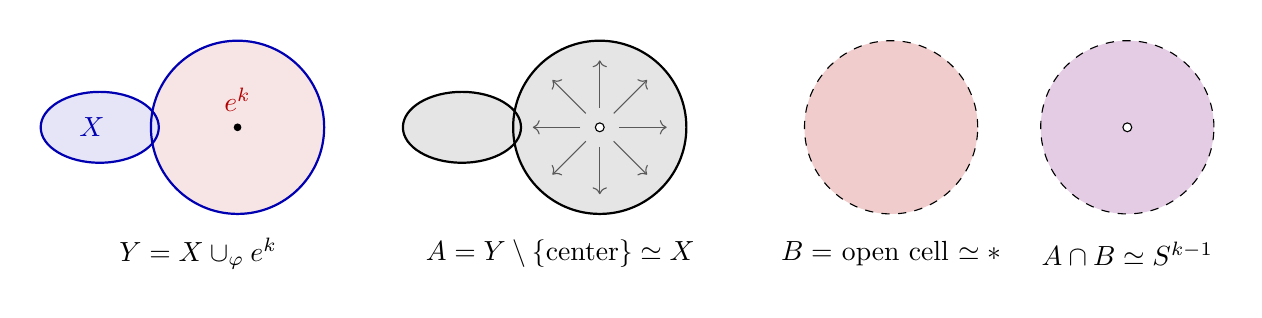
\begin{tikzpicture}
% panel Y
\begin{scope}
\fill[c2!10] (0,0) circle(1.1);
\draw[thick,c1,fill=c1!10] (-1.75,0) ellipse(0.75 and 0.45);
\draw[thick,c1] (0,0) circle(1.1);
\node[c1] at (-1.85,0){$X$}; \node[c2] at (0,0.35){$e^k$}; \fill (0,0) circle(1.4pt);
\node at (-0.5,-1.6){$Y=X\cup_\varphi e^k$};
\end{scope}
% panel A
\begin{scope}[xshift=4.6cm]
\fill[gray!20] (0,0) circle(1.1); \draw[thick,fill=gray!20] (-1.75,0) ellipse(0.75 and 0.45);
\draw[thick] (0,0) circle(1.1);
\draw[fill=white] (0,0) circle(1.6pt);
\foreach \t in {0,45,...,315} \draw[->,gray!70!black] (\t:0.25)--(\t:0.85);
\node at (-0.5,-1.6){$A=Y\setminus\{\text{center}\}\simeq X$};
\end{scope}
% panel B
\begin{scope}[xshift=8.3cm]
\fill[c2!20] (0,0) circle(1.1); \draw[dashed] (0,0) circle(1.1);
\node at (0,-1.6){$B=$ open cell $\simeq *$};
\end{scope}
% panel AB
\begin{scope}[xshift=11.3cm]
\fill[violet!20] (0,0) circle(1.1); \draw[dashed] (0,0) circle(1.1); \draw[fill=white] (0,0) circle(1.6pt);
\node at (0,-1.6){$A\cap B\simeq S^{k-1}$};
\end{scope}
\end{tikzpicture}\end{document}
